\documentclass[8pt]{beamer}

\usepackage{pgf,tikz}
\usetikzlibrary{shapes,snakes}
%\usetheme{Ilmenau}
\usetheme{Antibes}
%\usetheme{JuanLesPins}
%\usetheme{Darmstadt}
\usecolortheme{spruce}
\usepackage{amsmath}
\usepackage{tikz}
\usepackage{beamerfoils}
\usepackage{pgf}
\usepackage[table]{xcolor}
\usepackage{svg}
\usepackage{graphicx}
\usepackage{tikz}
% Preamble (add these if not already in your doc)
\usepackage{booktabs, makecell, tabularx}
% \renewcommand\theadfont{\itshape\normalsize}
% \renewcommand\theadgape{}
\renewcommand{\arraystretch}{1.25} % optional: a bit more row height
\usepackage{nameref}
\usepackage{hyperref}
\pdfstringdefDisableCommands{%
  \let\translate\relax
}

\usepackage[round,authoryear]{natbib}
\let\oldcitep\citep
\renewcommand{\citep}[1]{\textcolor{gray}{\oldcitep{#1}}}


\usetikzlibrary{positioning, arrows.meta, calc}

\definecolor{mygreen}{cmyk}{0.9,0.11,1,0.25}
\setbeamertemplate{blocks}[rounded][shadow=false]

% \addtobeamertemplate{block begin}{\pgfsetfillopacity{0.8}}{\pgfsetfillopacity{1}}

\setbeamercolor{structure}{fg=mygreen}
\setbeamercolor{title}{fg=ualberta_darkgreen, bg=ualberta_gold!50}

\setbeamercolor{block title}{
    fg=ualberta_darkgreen,
    bg=ualberta_gold!70
}
\setbeamerfont{block title}{series=\bfseries}
\setbeamercolor{block body}{parent=normal text,use=block title,bg=block title.bg!30!bg}
\setbeamercolor{block title example}{use=example text,fg=example text.fg,bg=example text.fg!50!bg}
\setbeamercolor{block body example}{parent=normal text,use=block title example,bg=block title example.bg!30!bg}

\definecolor{ualberta_darkgreen}{cmyk}{0.5806, 0, 0.3978, 0.6353}
\definecolor{ualberta_lightgreen}{cmyk}{0.4433, 0, 0.6118, 0.2392}
\definecolor{ualberta_verylightgreen}{cmyk}{0.0717, 0, 0.1435, 0.0706}
\definecolor{ualberta_gold}{cmyk}{0,0.1529,1,0.051}

\setbeamercolor{title in head/foot}{fg=ualberta_gold}
\setbeamercolor{section in head/foot}{fg=ualberta_verylightgreen}

\tikzstyle{block} = [rectangle, minimum width=2cm, minimum height=1cm,text centered, draw=black]
\tikzstyle{block_1} = [rectangle, minimum width=2cm, minimum height=1cm,text centered, draw=black, fill=blue!5]
\tikzstyle{block_2} = [rectangle, minimum width=2cm, minimum height=1cm,text centered, draw=black, fill=red!5]
\tikzstyle{arrow} = [thick,->,>=stealth]
\tikzstyle{arrow_2} = [very thick,->,>=stealth]
\tikzstyle{arrow_3} = [thick,->,>=stealth,dashed]
\tikzstyle{pfr} = [cylinder, draw, minimum height=4cm, minimum width=1cm, shape aspect=1, shape border rotate=180]
\usetikzlibrary{shapes.geometric}

% Insert spacing override here:
\makeatletter
\let\orig@itemize\itemize
\def\itemize{\orig@itemize\setlength\itemsep{10pt}\setlength\parsep{6pt}}
\makeatother

\MyLogo{
\pgfputat{\pgfxy(-8,6.8)}{\pgfbox[right,base]{
\includegraphics[height=1cm]{graph/UA_Logo_Green_RGB.png}}}
}


\title{\textbf{State-Delays in Chemical Engineering:\\A Control Framework for Distributed Parameter Systems}}
\author{Behrad `Brad' Moadeli}
\institute{Department of Chemical and Materials Engineering, University of Alberta\\Edmonton, Alberta, Canada}
% \centering
\date{
    % Department of Chemical and Materials Engineering\\University of Alberta\\ \vspace{3mm}
    September 5\textsuperscript{th}, 2025}

\setbeamertemplate{footline}[frame number]
\begin{document}
\LogoOn
\maketitle
\LogoOff
% \begin{frame}{Outline}
% \tableofcontents[hideallsubsections]
% \end{frame}
% \LogoOff











\section{Cahpter 1: Introduction}

\begin{frame}{Distributed Parameter Systems in Chemical Engineering}

\begin{columns}[c]
\column{0.48\textwidth}

\begin{itemize}
    \item Chemical processes $\rightarrow$ PDEs $\rightarrow$ \textbf{Distributed Parameter Systems (DPSs)}. \vspace{4mm}
    \item A canonical example $\rightarrow$ \textbf{Axial-Dispersion Tubular Reactors} $\rightarrow$ 2\textsuperscript{nd} order Parabolic PDEs. \vspace{4mm}
    \item Common in practice $\rightarrow$ \textbf{Recycle Streams} $\rightarrow$ Alter system dynamics. \citep{khatibi2021model}
\end{itemize}
\column{0.50\textwidth}

\begin{figure}[!htbp] 
    \centering
    \begin{tikzpicture}[scale=0.75, transform shape]
        \node (pfr) [cylinder, draw, minimum height=3cm, minimum width=1cm, shape aspect=1, shape border rotate=180, cylinder uses custom fill, cylinder end fill=ualberta_lightgreen, cylinder body fill=ualberta_verylightgreen] {\hspace{-0.2cm}$A \rightarrow Products$};
        \node (pfr_inlet) [circle, left of=pfr, xshift=-0.5cm, fill=black, draw, inner sep=0pt, minimum size=0.25cm, scale=0.5] {};
        \node (pfr_outlet) [circle, at={(pfr.east)}, shift={(-0.25cm,0)}, fill=black, draw, inner sep=0pt, minimum size=0.25cm, scale=0.5] {};
        \node (recycle_right) [circle, right of=pfr_outlet, fill=black, draw, inner sep=0pt, minimum size=0.25cm, scale=0.5] {};
        \node (recycle_left) [circle, left of=pfr_inlet, fill=black, draw, inner sep=0pt, minimum size=0.25cm, scale=0.5] {};
        \node[above of=pfr_inlet, xshift=1.25cm, node distance=0.75cm,] {$x(z, t)$};        
        \draw [arrow] (pfr_outlet) -- node[near end, above] {} ++(1.5,0);
        \draw [arrow] (pfr_inlet) ++(-1.5,0) coordinate(start) -- node[near start, above] {} (pfr_inlet);
        \draw [arrow] (recycle_right) -- ++(0,-1.00) -| (recycle_left);
    \end{tikzpicture}
    \caption{Axial tubular reactor with recycle stream.}
    \label{fig:reactor_scheme_1}
\end{figure}

\vspace{-2mm}
\begin{block}{Governing equation, general form}

\begin{equation} \label{eq:PDE_original_model_1}
    \begin{aligned}
        \partial_t{x}(\zeta, t) =& && \\
        &D \, \partial^2_{\zeta} x(\zeta, t) &&\text{Dispersion}\\
        - &v \, \partial_{\zeta} x(\zeta, t) &&\text{Convection} \\
        - &k \, x(\zeta, t) &&\text{Reaction}
    \end{aligned}
\end{equation}

\end{block}
\end{columns}
\end{frame}





\begin{frame}{Early Lumping vs. Late Lumping}
\begin{figure}
    \centering
    \resizebox{\textwidth}{!}{%
        \begin{tikzpicture}[
            block/.style={rectangle, draw, minimum width=4cm, minimum height=1.2cm, align=center},
            circleblock/.style={circle, draw, minimum size=2.2cm, align=center},
            ->, >=Stealth
        ]
            % Left circle
            \node[circleblock] (dps) {\textbf{Distributed}\\\textbf{Parameter}\\\textbf{System}};

            % Early lumping branch
            \node[block, right=0.8cm of dps, yshift=2.5cm] (early1) {Approximation to a\\Lumped Parameter System};
            \node[block, right=0.8cm of early1] (early2) {Control Theory for\\Finite Systems};

            % Late lumping branch
            \node[block, right=0.8cm of dps, yshift=-2.5cm, fill=ualberta_verylightgreen] (late1) {Control Theory for DPS};
            \node[block, right=0.8cm of late1, fill=ualberta_verylightgreen] (late2) {Approximation to obtain\\\textit{Numerical Solution}};

            % Centered implementation node
            \node[circleblock, anchor=west] at ($(early2.east) + (0.4cm, -2.5cm)$) (impl) {\textbf{Controller}\\\textbf{Implementation}};


            % Curved arrows from DPS
            \draw[->] (dps) to[bend left=20] node[midway, above, sloped] {\small Early Lumping} (early1.west);
            \draw[->] (dps) to[bend right=20] node[midway, below, sloped] {\small Late Lumping} (late1.west);

            % Horizontal arrows
            \draw[->] (early1) -- (early2);
            \draw[->] (late1) -- (late2);

            % Curved final arrows
            \draw[->] (early2.east) to[bend left=20] (impl);
            \draw[->] (late2.east) to[bend right=20] (impl);
        \end{tikzpicture}
    }
    \caption{Conceptual comparison between early and late lumping control strategies. \citep{guilhermethesis}}
\end{figure}
\end{frame}





\begin{frame}{Motivation: What's Missing?}
\begin{columns}[t]
\column{0.49\textwidth}
\textbf{Prior Work:}
\begin{itemize}
    \item Late lumping $\rightarrow$ well-developed for DPS control. \citep{curtainbook,Christofides2012book}
    \item Control of Parabolic PDEs $\rightarrow$ well-developed $\rightarrow$ e.g., Reactors w/o recycle. \citep{liu2014model,xu2017linear}
    \item Reactors with recycle studied \citep{khatibi2021model} $\rightarrow$ Instantaneous recycle
\end{itemize}

\column{0.49\textwidth}
\textbf{The Gap:}
\begin{itemize}
    \item Reality: Recycle takes time to travel.
    \item This travel time $\rightarrow$ \textbf{State Delay}.
    \item Unlike actuation/measurement delays $\rightarrow$ Absent in ChemEng DPS literature.
    \item No control framework to capture state delays in ChemEng DPS.
\end{itemize}
\end{columns}
\vspace{2mm}
\begin{block}{End Goal}
To develop a \textbf{modeling and control framework} via \textbf{late-lumping} approach, for chemical engineering \textbf{DPSs with state delays}, by studying axial dispersion tubular reactors as a \textit{general yet practically relevant} case.
\end{block}
\end{frame}

% \section{Model Representation}





\begin{frame}{Recycle-Induced State Delay: A Closer Look}
\begin{columns}[c]
\column{0.54\textwidth}
\vspace{-3mm}
\begin{figure}[!htbp] 
    \centering
    \begin{tikzpicture}[scale=0.75, transform shape]
        \node (pfr) [cylinder, draw, minimum height=3cm, minimum width=1cm, shape aspect=1, shape border rotate=180, cylinder uses custom fill, cylinder end fill=ualberta_lightgreen, cylinder body fill=ualberta_verylightgreen] {\hspace{-0.2cm}$A \rightarrow Products$};
        \node (pfr_inlet) [circle, left of=pfr, xshift=-0.5cm, fill=black, draw, inner sep=0pt, minimum size=0.25cm, scale=0.5] {};
        \node (pfr_outlet) [circle, at={(pfr.east)}, shift={(-0.25cm,0)}, fill=black, draw, inner sep=0pt, minimum size=0.25cm, scale=0.5] {};
        \node (recycle_right) [circle, right of=pfr_outlet, fill=black, draw, inner sep=0pt, minimum size=0.25cm, scale=0.5] {};
        \node (recycle_left) [circle, left of=pfr_inlet, fill=black, draw, inner sep=0pt, minimum size=0.25cm, scale=0.5] {};
        
        \draw[dotted, thick] ([yshift=0.5cm]pfr_inlet.center) -- node[at end, below, yshift=0.1cm] {$\zeta = 0$} ([yshift=-0.65cm]pfr_inlet.center);
        \draw[dotted, thick] ([yshift=0.5cm]pfr_outlet.center) -- node[at end, below, yshift=0.1cm] {$\zeta = 1$} ([yshift=-0.65cm]pfr_outlet.center);
        
        \node[below of=recycle_left, node distance=1.3cm, anchor=north west, xshift=-0.2cm]{$R \, c(1, t - \textcolor{ualberta_darkgreen}{\boldsymbol{\tau}})$};

        \node[above of=pfr_inlet, node distance=0.75cm,] {$c(0, t)$};
        \node[above of=pfr_outlet, node distance=0.75cm,] {$c(1, t)$};
        
        \draw [arrow_2] (pfr_outlet) -- node[near end, above] {$y(t)$} ++(2,0);
        \draw [arrow_2] (pfr_inlet) ++(-2,0) coordinate(start) -- node[near start, above] {$u(t)$} (pfr_inlet);
        \draw [arrow_2] (recycle_right) -- ++(0,-1.25) -| (recycle_left);
        
    \end{tikzpicture}
    \caption{Axial tubular reactor with recycle-induced state delay.}
    \label{fig:reactor_scheme}
    % \pdfbookmark[2]{Figure: Reactor Scheme}{fig:reactor_scheme}
\end{figure}
\column{0.44\textwidth}
\textbf{General Setup:}\vspace{2mm}
\begin{itemize}
    \item 2\textsuperscript{nd} order parabolic PDE.
    \item Danckwerts-type boundary conditions.
\end{itemize}
\end{columns}

\begin{block}{Governing PDE (Isothermal)}
\begin{equation} \label{eq:PDE_original_model}
    \begin{aligned}
        \partial_t{c}(\zeta, t) &= D \, \partial^2_{\zeta} c(\zeta, t) - v \, \partial_{\zeta} c(\zeta, t) - k_r \, c(\zeta, t) \\
        &\begin{cases}
            \begin{aligned}
                D \, \partial_{\zeta} c(0, t) - v \, c(0, t) &= -v \left[ R \, c(1, t - \textcolor{ualberta_darkgreen}{\boldsymbol{\tau}}) + (1 - R) \, u(t) \right] \\
                \partial_{\zeta} c(1, t) &= 0 \\
                y(t) &= c(1, t)
            \end{aligned}
        \end{cases}
    \end{aligned}
\end{equation}
\end{block}
\end{frame}






\begin{frame}{Key Novelty: Delay as a Transport PDE}
\begin{columns}[c]
\column{0.44\textwidth}

\begin{itemize}
    \item A transport PDE over \( \zeta \in [0, 1] \):
    \[
        \frac{\partial x}{\partial t} - \frac{1}{\tau} \frac{\partial x}{\partial \zeta} = 0, \quad
        x(0, t) = u(t)
    \]
    \item Describes propagation of input \( u(t) \) with delay:
    \[
        x(1, t) = u(t - \tau)
    \]
    \item Delay emerges as \textbf{residence time} across domain.
    \item Foundation for modeling \textbf{state delay} as a PDE. \citep{krstic2009book}
\end{itemize}

\column{0.54\textwidth}
\begin{figure}
    \centering
    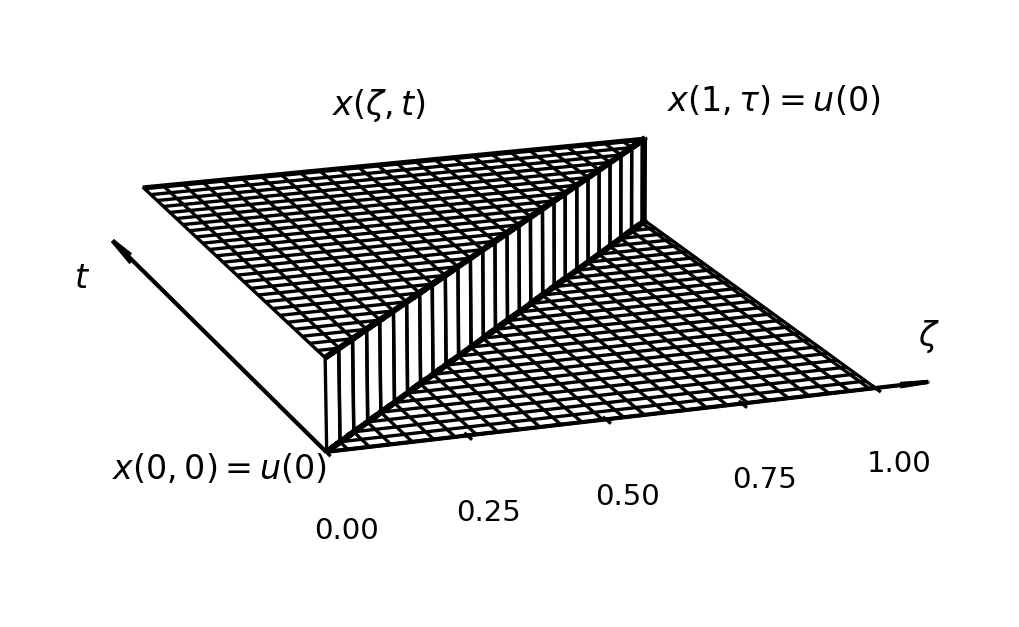
\includegraphics[width=\linewidth]{figures/transport_delay.png}
    \caption{A step input propagates spatially and appears at the outlet with delay \(\tau\).}
\end{figure}
\end{columns}

\begin{block}{Coupled PDE System}
    Results in a \textbf{time-invariant} representation of the system, suitable for \textbf{infinite-dimensional control theory}.
\end{block}

\end{frame}






\begin{frame}{Overall Trajectory}
\begin{small}
\begin{table}[h!]
\centering
\caption{Thesis trajectory across Chapters 2--4.}
\label{tab:chapters_summary}
\begin{tabularx}{0.9\textwidth}{%
  >{\raggedright\arraybackslash}X
  >{\raggedright\arraybackslash}X
  >{\raggedright\arraybackslash}X
  >{\raggedright\arraybackslash}X
  >{\raggedright\arraybackslash}X
  >{\raggedright\arraybackslash}X}
\toprule
\thead{Thesis\\chapter} &
\thead{Model\\assumption} &
\thead{Temporal\\domain} &
\thead{Controller\\strategy} &
\thead{Estimation\\method} &
\thead{Publications} \\
\midrule
Chapter 2 &
Isothermal &
Continuous-time &
LQR (unconstrained) &
Luenberger observer (unconstrained) &
\citep{moadeli2025optimal} \\
\addlinespace
Chapter 3 &
Isothermal &
Discrete-time &
MPC (constrained) &
Luenberger observer (unconstrained) &
\citep{moadeli2025acc, moadeli2025ecc} \\
\addlinespace
Chapter 4 &
Non-isothermal &
Discrete-time &
MPC (constrained) &
MHE (constrained) &
\citep{moadeli2025advanced} \\
\bottomrule
\end{tabularx}
\end{table}
\end{small}
\end{frame}


\section{Chapter 2: Continuous-time Estimation and Optimal Control for the Isothermal System}


\begin{frame}{Chapter 2: Continuous-time Estimation and Optimal Control for the Isothermal System}
\begin{small}
\begin{table}[h!]
\centering
\caption{Thesis trajectory across Chapters 2--4.}
\label{tab:chapters_summary_ch2}
\begin{tabularx}{0.9\textwidth}{%
  >{\raggedright\arraybackslash}X
  >{\raggedright\arraybackslash}X
  >{\raggedright\arraybackslash}X
  >{\raggedright\arraybackslash}X
  >{\raggedright\arraybackslash}X
  >{\raggedright\arraybackslash}X}
\toprule
\thead{Thesis\\chapter} &
\thead{Model\\assumption} &
\thead{Temporal\\domain} &
\thead{Controller\\strategy} &
\thead{Estimation\\method} &
\thead{Publications} \\
\midrule
\rowcolor{ualberta_verylightgreen}
Chapter 2 &
Isothermal &
Continuous-time &
LQR (unconstrained) &
Luenberger observer (unconstrained) &
\citep{moadeli2025optimal} \\
\addlinespace
Chapter 3 &
Isothermal &
Discrete-time &
MPC (constrained) &
Luenberger observer (unconstrained) &
\citep{moadeli2025acc, moadeli2025ecc} \\
\addlinespace
Chapter 4 &
Non-isothermal &
Discrete-time &
MPC (constrained) &
MHE (constrained) &
\citep{moadeli2025advanced} \\
\bottomrule
\end{tabularx}
\end{table}
\end{small}
\end{frame}








\begin{frame}{Infinite-Dimensional State-Space Representation}
    
\begin{block}{System Dynamics}
    \begin{equation} \label{eq:state_space}
        \dot{x}(\zeta, t) = A x(\zeta, t) + B u(t); \qquad
        y(t) = C x(\zeta, t)
    \end{equation}
\end{block}
    
\begin{columns}[c]
\column{0.48\textwidth}

\begin{equation} \label{eq:operator_A}
    \begin{aligned}
        A &:=
        \begin{bmatrix}
            D \partial_{\zeta \zeta} - v \partial_\zeta - k_r & 0 \\
            0 & \frac{1}{\tau} \partial_\zeta
        \end{bmatrix} \\[5mm]
        \mathcal{D}(A) =& \Bigl\{ x(\zeta) = [x_1(\zeta), x_2(\zeta)]^T \in X:\\[1mm]
        &x(\zeta), \partial_\zeta x(\zeta), \partial_{\zeta \zeta} x(\zeta) \quad \mathrm{a.c.},\\[1mm]
        &D \partial_\zeta x_1(0) - v x_1(0) = -v R x_2(0),\\[1mm]
        &\partial_\zeta x_1(1) = 0,
        x_1(1) = x_2(1) \Bigr\}\\
        % B &:=
        % \begin{bmatrix}
        %     \delta(\zeta) \\
        %     0
        % \end{bmatrix} v(1-R) \\
        % C &:=
        % \begin{bmatrix}
        %     \int_0^1 \delta(\zeta-1) (\cdot) d\zeta & 0
        % \end{bmatrix} \\
        % D &= 0
        % \mathcal{D}(C) &= \mathcal{D}(A)
    \end{aligned}
\end{equation}


\column{0.50\textwidth}

\begin{equation} \label{eq:operator_B_C_D}
    \begin{aligned}
        x &:= \begin{bmatrix} x_1 \\ x_2 \end{bmatrix} \in L^2[0,1] \times L^2[0,1]\\[6mm]
        % A &:=
        % \begin{bmatrix}
        %     D \partial_{\zeta \zeta} - v \partial_\zeta + k_r & 0 \\
        %     0 & \frac{1}{\tau} \partial_\zeta
        % \end{bmatrix} \\
        % \mathcal{D}(A) =& \Bigl\{ x(\zeta) = [x_1(\zeta), x_2(\zeta)]^T \in X:\\
        % &x(\zeta), \partial_\zeta x(\zeta), \partial_{\zeta \zeta} x(\zeta) \quad \mathrm{a.c.},\\
        % &D \partial_\zeta x_1(0) - v x_1(0) = -v R x_2(0),\\
        % &\partial_\zeta x_1(1) = 0,
        % x_1(1) = x_2(1) \Bigr\}\\
        B &:=
        \begin{bmatrix}
            \delta(\zeta) \\
            0
        \end{bmatrix} v(1-R) \\[3mm]
        C &:=
        \begin{bmatrix}
            \int_0^1 \delta(\zeta-1) (\cdot) d\zeta & 0
        \end{bmatrix} \\[3mm]
        D &= 0
        % \mathcal{D}(C) &= \mathcal{D}(A)
    \end{aligned}
\end{equation}
\end{columns}
\end{frame}

\begin{frame}{Eigenvalue Distribution: System is Unstable}

\begin{columns}[c]
\column{0.5\textwidth}

\begin{itemize}
    \item Spectrum of system generator $\sigma(A$) determines open-loop stability.
    \item Characteristics equation $det(\lambda_i-A) = 0$ is solved to obtain eigenvalues.
    \item Direct analytical solution is impractical—solved numerically.
    \item Result: eigenvalues with \textbf{positive real parts} → \textcolor{red}{open-loop unstable}.
    \item Parameters used to obtain the eigenvalue distribution are given in Table~\ref{tab:pars_1} in \nameref{tab:pars_1}.
\end{itemize}

\column{0.5\textwidth}
\begin{figure}
    \centering
    \includesvg[width=0.75\linewidth]{Figures/eig_val_dist_R_0.3.svg}
    \caption{Eigenvalue distribution of system operator \( A \)}
\end{figure}
\end{columns}
\end{frame}



% ===== Slide 3: LQR via Operator Riccati → Full-State Gain =====
\begin{frame}{LQR: Operator Riccati Equation}
\begin{columns}[t]
\column{0.44\textwidth}

\begin{itemize}
  \item Cost: $J=\int_0^\infty \langle x,{Q}x\rangle + \langle u,{R}u\rangle\,ds$.
  \item Solve operator Riccati for ${\Pi}$; truncate in biorthogonal basis to get matrix Riccati for $P=[p_{ij}]$.
\end{itemize}
\small
\begin{align*}
u(t) &= -\langle k_{\mathrm{ric}}(\zeta),\,x(\zeta,t)\rangle
= -{B}^* {\Pi}x(\zeta,t),\\
k_{\mathrm{ric}}(\zeta) &\equiv \sum_{i=1}^{N}\sum_{j=1}^{N} p_{i,j}\,\gamma_i\,\overline{\psi_j}(\zeta)
% \quad\text{(\textit{cf.} \eqref{eq:1_fullstate_gain}).}
\end{align*}
\column{0.54\textwidth}
\begin{figure}
    \centering
    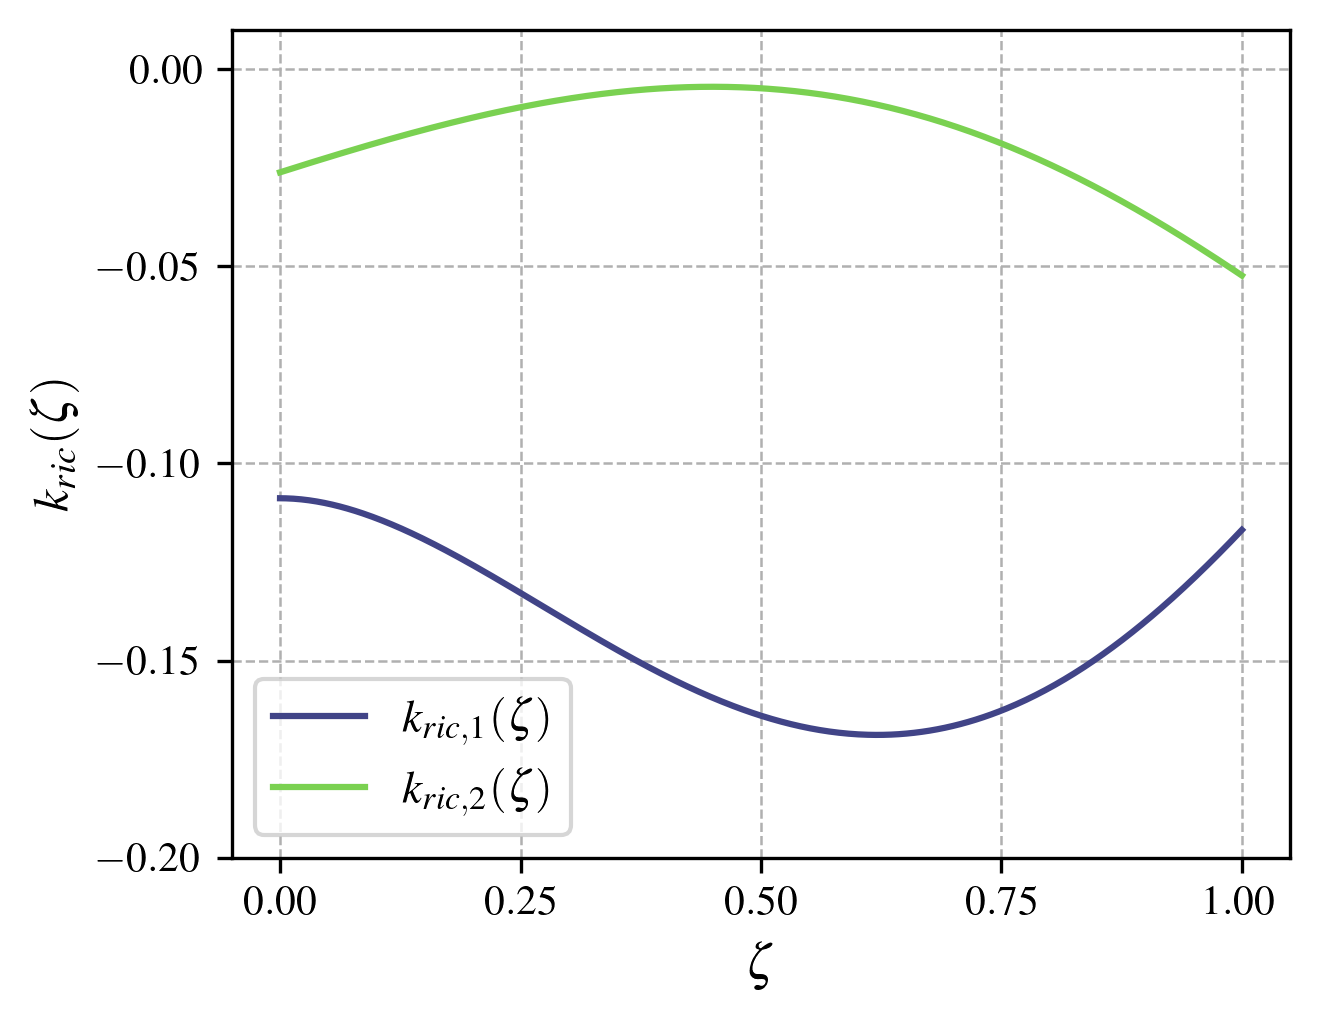
\includegraphics[width=0.85\textwidth]{figures/k_3.png}\\[-1em]
    \caption{$k_{\mathrm{ric}}(\zeta)$, $N{=}3$}
\end{figure}
\end{columns}

% {\footnotesize (Weights as set in \texttt{03\_control.tex}; block diagram shown in Fig.~\ref{fig:1_block_diagram}.)}
\end{frame}

% ===== Slide 4: Output-Feedback Observer (Pole Placement) =====
\begin{frame}{Observer Design and Pole Placement}
\begin{itemize}
  \item Output operator (point measurement): 
  $\displaystyle {C}=\begin{bmatrix}\int_0^1\delta(\zeta-1)(\cdot)\,d\zeta,\; 0\end{bmatrix}$.
  \item Choose ${L}(\zeta)$ s.t. ${A}-{L}{C}$ has desired eigenvalues (to the left of regulator poles).
  \item Error dynamics: $\dot e=({A}-{L}{C})e$.
\end{itemize}
\centering
\includesvg[inkscapelatex=false,width=0.43\textwidth]{figures/L.svg}\hfill
\includesvg[inkscapelatex=false,width=0.48\textwidth]{figures/pole_placement.svg}\\
{\footnotesize Figure: Observer gain profile and closed-loop eigenvalue placement.}
\end{frame}

% ===== Slide 5: Results — Stabilization (Full-State \& Observer) =====
\begin{frame}{Results: Stabilization Achieved (FDM validation)}
\begin{columns}[t]
\column{0.48\textwidth}
\begin{itemize}
  \item Both full-state LQR and observer-based output feedback stabilize the PDE system (finite-difference validation).
  \item Observer-based loop is slightly more sluggish but robust and stable.
  \item Delay sensitivity: maintains stability for moderate $\tau$ mismatch used in design.
\end{itemize}

\column{0.48\textwidth}
\begin{figure}
    \centering
% \begin{minipage}{0.48\textwidth}\centering
% 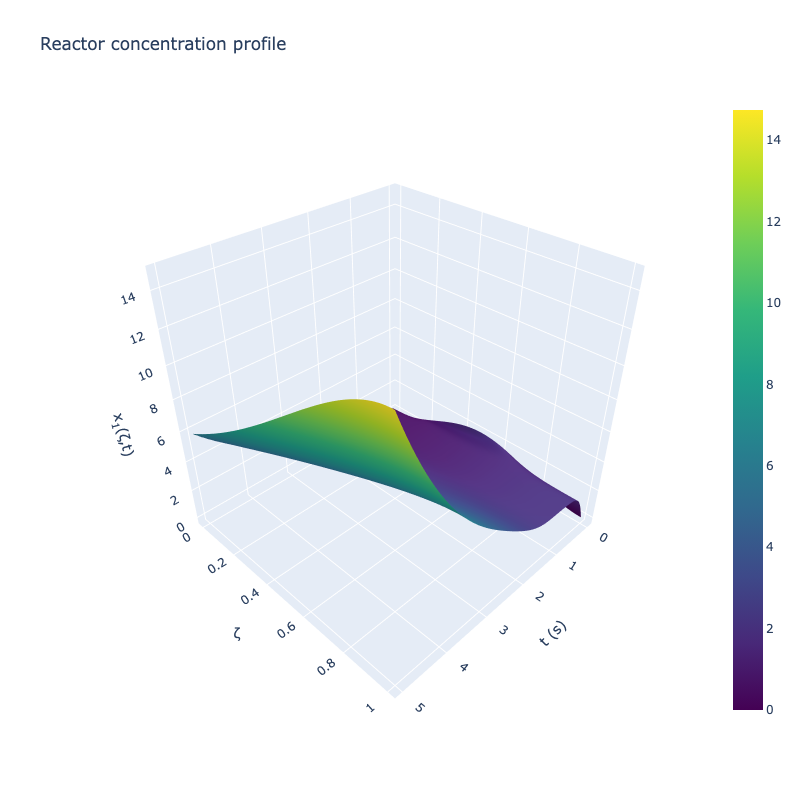
\includegraphics[width=\textwidth]{figures/3D_x1_openloop.png}\\[-0.2em]
% {\footnotesize Open-loop $x_1(\zeta,t)$}
% \end{minipage}\hfill
    \includesvg[width=\textwidth]{figures/3D_x1_L_k7.svg}\\[-0.2em]
    \caption{Closed-loop $x_1(\zeta,t)$ (LQR)}
\end{figure}
\vspace{0.4em}
% \includesvg[inkscapelatex=false,width=0.72\textwidth]{figures/y_vs_t.svg}\\
% {\footnotesize Output $y(t)$ under observer-based control for different $\tau$ (design $\tau$ indicated).}
\end{columns}
\end{frame}









\section{Chapter 3: Discrete-time Estimation and Model Predictive Control for the Isothermal System}


\begin{frame}{Chapter 3: Discrete-time Estimation and Model Predictive Control for the Isothermal System}
\begin{small}
\begin{table}[h!]
\centering
\caption{Thesis trajectory across Chapters 2--4.}
\label{tab:chapters_summary_ch3}
\begin{tabularx}{0.9\textwidth}{%
  >{\raggedright\arraybackslash}X
  >{\raggedright\arraybackslash}X
  >{\raggedright\arraybackslash}X
  >{\raggedright\arraybackslash}X
  >{\raggedright\arraybackslash}X
  >{\raggedright\arraybackslash}X}
\toprule
\thead{Thesis\\chapter} &
\thead{Model\\assumption} &
\thead{Temporal\\domain} &
\thead{Controller\\strategy} &
\thead{Estimation\\method} &
\thead{Publications} \\
\midrule
Chapter 2 &
Isothermal &
Continuous-time &
LQR (unconstrained) &
Luenberger observer (unconstrained) &
\citep{moadeli2025optimal} \\
\addlinespace
\rowcolor{ualberta_verylightgreen}
Chapter 3 &
Isothermal &
Discrete-time &
MPC (constrained) &
Luenberger observer (unconstrained) &
\citep{moadeli2025acc, moadeli2025ecc} \\
\addlinespace
Chapter 4 &
Non-isothermal &
Discrete-time &
MPC (constrained) &
MHE (constrained) &
\citep{moadeli2025advanced} \\
\bottomrule
\end{tabularx}
\end{table}
\end{small}
\end{frame}







\section{Cayley-Tustin Time-Discretization}

\begin{frame}{Cayley-Tustin Time-Discretization}

\begin{columns}[c]
\column{0.48\textwidth}

\begin{block}{Discrete-time System}
\begin{equation} \label{eq:state_space_dt}
\begin{aligned}
    \dot{x}(\zeta, k) &= A_d x(\zeta, k{-}1) + B_d u(k) \\
    y(k) &= C_d x(\zeta, k{-}1) + D_d u(k)
\end{aligned}
\end{equation}
\end{block}
    
\begin{itemize}
    \item Discretization is needed for \\\textbf{digital controller implementation}.
    \item Cayley-Tustin discretization preserves:\\ \,
    \begin{itemize}\setlength\itemsep{4pt}
        \item System's \textbf{infinite-dimensional structure}
        \item \textbf{Stability} and \textbf{controllability}
        \item \dots
    \end{itemize}
\end{itemize}


\column{0.48\textwidth}

\begin{block}{continuous- to discrete-time mapping}
\vspace{1mm}
\begin{equation} \label{eq:ct_to_dt}
\begin{aligned}
    A_d &= - I + 2\alpha {R}(\alpha, A), \\
    B_d &= \sqrt{2\alpha} {R}(\alpha, A) B, \\
    C_d &= \sqrt{2\alpha} C {R}(\alpha, A), \\
    D_d &= C {R}(\alpha, A) B
\end{aligned}
\end{equation}
\vspace{1mm}
\end{block}
\vspace{2mm}
\begin{itemize}
    \item ${R}(\alpha, A) := \left[ \alpha I - A \right]^{-1}$ is the \textbf{resolvent operator} of system generator $A$.
    \item \( \alpha = \frac{2}{\Delta t} \), where \( \Delta t \) is the sampling time.
\end{itemize}
    
\end{columns}
\end{frame}

\begin{frame}{Resolvent Operator: Role and Procedure}
\begin{itemize}
    \item To follow the \textbf{late-lumping} approach, it is crucial to obtain a \textbf{closed-form representation} of the resolvent operator, which bridges the continuous- and discrete-time domains.
    \item This is done by interpreting the resolvent as a \textbf{mapping} from either \textit{initial conditions} or \textit{inputs} to the \textit{Laplace-transformed state}.
\end{itemize}

\begin{columns}[c]
\column{0.52\textwidth}

\begin{block}{Laplace Transform}
\begin{small}
\begin{equation} \label{eq:resolvent}
\begin{aligned}
    \dot{x}(\zeta, t) &= A x(\zeta, t) + B u(t) \xrightarrow{\mathcal{L}}\\
    s x(\zeta,s) - x(\zeta,0) &= A x(\zeta,s) + B U(s)\\
    &\hspace{-7em}
    \begin{cases}
        \begin{aligned}
            u = 0 &\rightarrow x = {R}(s, A) \, x(0) \\
            x(0) = 0 &\rightarrow x = {R}(s, A) \, B U(s)
        \end{aligned}
    \end{cases}
\end{aligned}
\end{equation}
\end{small}
\end{block}


\column{0.46\textwidth}
\vspace{6mm}\\
\textbf{To compute \({R}(s, A)\):}
\begin{small}
\begin{itemize}\setlength\itemsep{4pt}
    \item Apply Laplace transform to the PDE system.
    \item Reformulate as a spatial ODE in \(\zeta\), solve using \(e^{P(s)\zeta}\).
    \item Enforce boundary conditions to determine \(\tilde{X}(0,s)\).
    \item Combine terms to obtain closed-form \({R}(s, A)\).
\end{itemize}
\end{small}
\end{columns}
\begin{center}
    \small See slide~\ref{app:resolvent} in \nameref{app:resolvent} for full derivation
\end{center}
\end{frame}




\begin{frame}{Continuous-Time Luenberger Observer Design}
\begin{columns}[t]
\column{0.46\textwidth}
\begin{itemize}
    \item State measurements in DPSs are infeasible: states are distributed over space. A \textbf{Luenberger observer} reconstructs full state using output \( y(t) \).
    \item Observer dynamics:
\end{itemize}
\begin{small}
\begin{equation}
    \begin{aligned}
    \dot{\hat{x}}(\zeta, t) &= A \hat{x}(\zeta, t) + B u(t)\\
    &+ {L}_c \left[y(t) - \hat{y}(t)\right], \\[1mm]
    \hat{y}(t) &= C \hat{x}(\zeta, t)
    \end{aligned}
\end{equation}
\end{small}
\begin{itemize}
    \item Estimation error: \( e(\zeta, t) = x(\zeta, t) - \hat{x}(\zeta, t) \), evolves as \( \dot{e}(\zeta, t) = (A - {L}_c C) e(\zeta, t) = A_o  e(\zeta, t) \).
\end{itemize}
\column{0.52\textwidth}
\begin{itemize}
    \item Gain \( {L}_c = f(\zeta, l_{\text{obs}}) \) is tuned to place $A_o$ eigenvalues in left half-plane.
\end{itemize}
\begin{figure}
    \centering
    \includesvg[width=0.95\linewidth]{Figures/obs_lambda.svg}
    \caption{The effect of various observer gains ${L}_c = f(\zeta, l_{obs})$ on the eigenvalues of state reconstruction error dynamics $\lambda_o$.}
\end{figure}
\end{columns}
\end{frame}

\begin{frame}{Discrete-Time Observer via Cayley-Tustin}
\begin{itemize}
    \item Cayley-Tustin time discretization yields a DT observer in the form:
\end{itemize}
\begin{small}
\begin{equation} \label{eq:observer_discrete}
    \begin{aligned}
        \hat{x}(\zeta, k) &= A_d \hat{x}(\zeta, k-1) + B_d u(k) + {L}_d [y(k) - \hat{y}(k)] \\
        \hat{y}(k) &= C_{d,o} \hat{x}(\zeta, k-1) + D_{d,o} u(k) + {M}_{d,o} y(k)
    \end{aligned}
\end{equation}
\end{small}
\begin{itemize}
    \item with the following continuous- to discrete-time mapping:
\begin{small}
\begin{equation} \label{eq:observer_discrete_CDLM}
    \begin{aligned}
        C_{d,o} (\cdot) &= \sqrt{2\alpha} \left[ I + C (\alpha I - A) {L}_c \right]^{-1} C {R}(\alpha, A) (\cdot) \\
        D_{d,o} &= \left[ I + C (\alpha I - A) {L}_c \right]^{-1} C {R}(\alpha, A) B \\
        {M}_{d,o} &= \left[ I + C {R}(\alpha, A) {L}_c \right]^{-1} C {R}(\alpha, A) {L}_c \\
        {L}_d &= \sqrt{2\alpha} {R}(\alpha, A) {L}_c \\
    \end{aligned}
\end{equation}
\end{small}
    \item Resulting DT error dynamics are stable \textbf{if CT observer is stable} \citep{xu2016state}.
\end{itemize}

\begin{block}{Key Point}
\textbf{No spatial discretization}: Observer is constructed using the same resolvent operator.
\end{block}
\end{frame}

\begin{frame}{MPC Architecture: Output-Feedback Loop}

\begin{itemize}
    \item Observer reconstructs \( \hat{x}(k) \), passed to MPC at each time step.
    \item MPC uses predicted future states and solves constrained QP over a finite horizon.
    \item Only the first control input is applied → \textbf{receding horizon}.
\end{itemize}

\begin{figure}[!htbp]
    \centering
    \begin{tikzpicture}[node distance=2cm, scale=0.75, transform shape]
        \node (plant) [block, minimum width=3cm] {Plant};
        \node (regulator) [block, below of=plant, xshift=-1cm, yshift=-1cm, fill=ualberta_gold!30] {MPC};
        \node (observer) [block, below of=plant, xshift=1cm, yshift=0.5cm, fill=ualberta_verylightgreen] {Observer};
        \draw [arrow] (plant.east) -- node[midway, above] {$y(k)$} ++(2,0);
        \draw [arrow] (plant.east) ++(1,0) |- (observer.east);
        \draw [arrow] (observer.south) -- ++(0,-1) node[midway, right] {$\hat{{x}}(\zeta,k)$} -- (regulator.east);    
        \draw [arrow] (regulator.west) -- ++(-1,0) |- (plant.west);
        \draw [arrow] (regulator.west) ++(-1,1.5) coordinate(start) -- node[near start, left, xshift=-0.75cm] {$u(k)$} (observer.west);
    \end{tikzpicture}
    \caption{Block diagram representation of the observer-based MPC.}
    \label{fig:block_diagram}
\end{figure}

\end{frame}

\begin{frame}{MPC Formulation with Terminal Projection}
\begin{columns}[t]
\column{0.48\textwidth}
\begin{itemize}
    \item Finite-horizon MPC:
\end{itemize}
\begin{equation} \label{eq:MPC_finite_time}
    \begin{aligned}
        \min_{U} \quad \sum_{l=0}^{N-1} &\langle \hat{x}(\zeta, k+l | k), {Q} \hat{x}(\zeta, k+l | k) \rangle \\
        + &\langle u(k+l+1 | k), {F} u(k+l+1|k) \rangle \\
        + &\langle \hat{x}(\zeta, k+N | k), {P} \hat{x}(\zeta, k+N | k) \rangle \\[3mm]
        \text{s.t.} \quad &\hat{x}(\zeta, k+l | k) =\\
        & A_d \hat{x}(\zeta, k+l-1 | k) + B_d u(k+l | k) \\
        &u^{min} \leq u(k+l | k) \leq u^{max} \\
        & \textcolor{ualberta_darkgreen}{\langle \hat{x}(\zeta, k+N | k), {\phi_u}(\zeta) \rangle = 0}
    \end{aligned}
\end{equation}
\vspace{-2mm}
\begin{itemize}
    \item ${P}$ is the \textbf{terminal cost operator} obtained as the solution to the \textit{discrete-time Lyapunov} equation:
\end{itemize}
\column{0.50\textwidth}
\begin{equation} \label{eq:terminal_cost}
    {P} (\cdot) = \sum_{m=0}^{\infty} \sum_{n=0}^{\infty} 
    -\frac{
        \langle {\phi_m} , {Q} {\psi_n} \rangle
    }{
        \lambda_m + \overline{\lambda_n}
    }
    \langle (\cdot) , {\psi_n} \rangle {\phi_m}
\end{equation}
\begin{itemize}
    \item The constrained QP is \textbf{convex} only if ${P}$ is \textbf{positive definite}.
    \item ${P}$ is {positive definite} only if the terminal state $\hat{x}(\zeta, k+N | k)$ is in a \textbf{stable subspace}.
    \item A \textcolor{ualberta_darkgreen}{\textbf{terminal constraint}} is introduced as an \textit{equality constraint} by setting the \textbf{projection of the terminal state} onto the \textbf{unstable subspace} of the system equal to zero.
\end{itemize}
\end{columns}
\end{frame}






\begin{frame}{Results: Stabilization under Observer-based MPC}
\begin{columns}[t]
\column{0.46\textwidth}
\begin{itemize}
    \item Initial condition: \( x_1(\zeta,0) = \sin^2(\pi \zeta) \), \( x_2(\zeta,0) = 0 \)
    \item Sampling time \( \Delta t = 20 \) s
    \item Horizon length \( N = 9 \)
    \item Input bounds: \( 0 \leq u(t) \leq 0.15 \)
\end{itemize}

\begin{figure}
    \centering
    \includesvg[width=0.9\linewidth]{Figures/input.svg}\vspace{-2em}
    \caption{Control input and reactor output under MPC.}
\end{figure}

\column{0.54\textwidth}
\vspace{-5mm}
\begin{figure}
    \centering
    \includesvg[width=0.9\linewidth]{Figures/closedloop_response.svg}\vspace{-2em}
    \caption{Stabilized concentration profile under observer-MPC.}
\end{figure}
% \vspace{-7mm}
% \begin{figure}
%     \centering
%     \includesvg[width=0.9\linewidth]{Figures/observation_error.svg}\vspace{-2em}
%     \caption{Decay of estimation error along the reactor.}
% \end{figure}


\end{columns}

\end{frame}





\section{Chapter 4: Non-isothermal System---Moving Horizon Estimation and Model Predictive Control}


\begin{frame}{Chapter 4: Non-isothermal System---Moving Horizon Estimation and Model Predictive Control}
\begin{small}
\begin{table}[h!]
\centering
\caption{Thesis trajectory across Chapters 2--4.}
\label{tab:chapters_summary_ch4}
\begin{tabularx}{0.9\textwidth}{%
  >{\raggedright\arraybackslash}X
  >{\raggedright\arraybackslash}X
  >{\raggedright\arraybackslash}X
  >{\raggedright\arraybackslash}X
  >{\raggedright\arraybackslash}X
  >{\raggedright\arraybackslash}X}
\toprule
\thead{Thesis\\chapter} &
\thead{Model\\assumption} &
\thead{Temporal\\domain} &
\thead{Controller\\strategy} &
\thead{Estimation\\method} &
\thead{Publications} \\
\midrule
Chapter 2 &
Isothermal &
Continuous-time &
LQR (unconstrained) &
Luenberger observer (unconstrained) &
\citep{moadeli2025optimal} \\
\addlinespace
Chapter 3 &
Isothermal &
Discrete-time &
MPC (constrained) &
Luenberger observer (unconstrained) &
\citep{moadeli2025acc, moadeli2025ecc} \\
\addlinespace
\rowcolor{ualberta_verylightgreen}
Chapter 4 &
Non-isothermal &
Discrete-time &
MPC (constrained) &
MHE (constrained) &
\citep{moadeli2025advanced} \\
\bottomrule
\end{tabularx}
\end{table}
\end{small}
\end{frame}


\begin{frame}{Non-isothermal System Model}

\begin{figure}
    \centering
    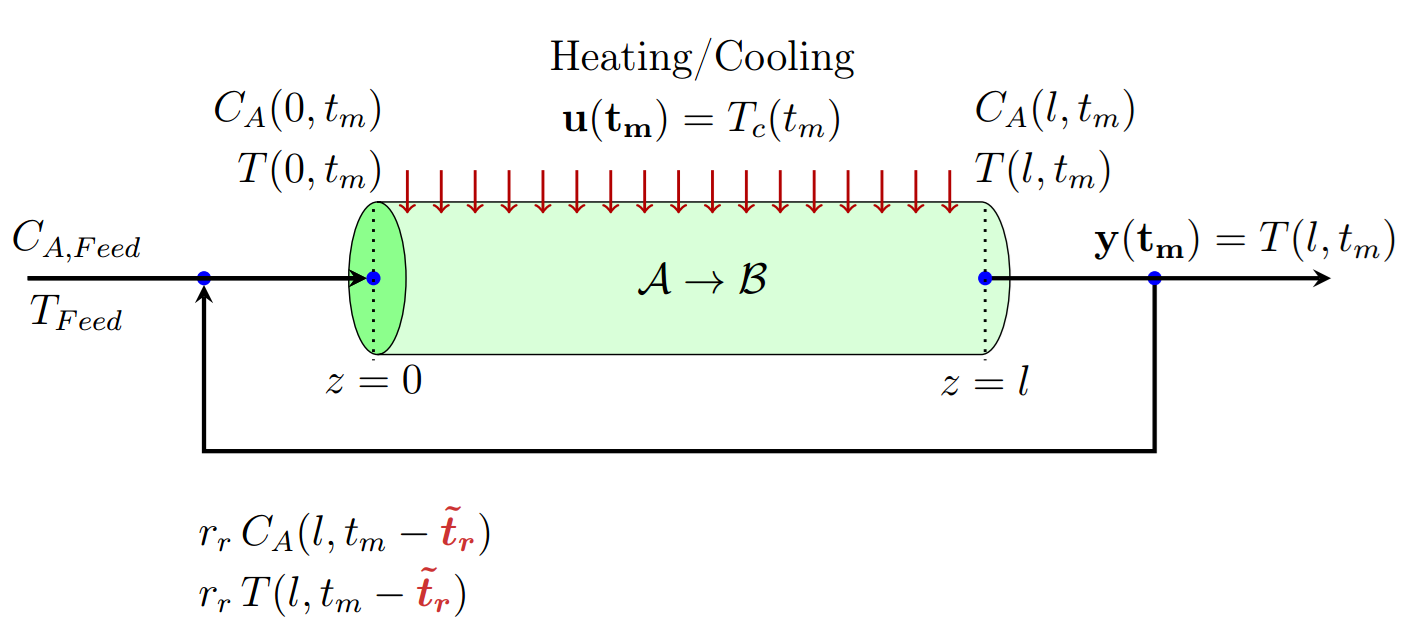
\includegraphics[width=0.6\textwidth]{figures/noniso_reactor.png}\vspace{-2mm}
    \caption{Non-isothermal system schematic.}
\end{figure}

\small
\textbf{States:} $x=[m_1(\zeta,t),\,m_2(\zeta,t),\,m_3(\zeta,t),\,m_4(\zeta,t)]^\top$ (reactor concentration/temperature and their recycle-line counterparts). \\
\textbf{Input:} wall/jacket temperature $u(t)=T_w(t)$. \ \ \textbf{Output:} $y(t)=m_2(1,t)$ (outlet temperature).\\[0.35em]
\begin{align*}
\partial_t m_1 &= \tfrac{1}{Pe_m}\partial_{\zeta\zeta} m_1 - \partial_\zeta m_1 
      + k_a\!\left(1-m_1\right)e^{\frac{\eta m_2}{1+m_2}}, \\
\partial_t m_2 &= \tfrac{1}{Pe_T}\partial_{\zeta\zeta} m_2 - \partial_\zeta m_2 
      + \alpha k_a\!\left(1-m_1\right)e^{\frac{\eta m_2}{1+m_2}} + \sigma\!\left(T_w(t)-m_2\right), \\
\partial_t m_3 &= \tfrac{1}{\tau}\partial_\zeta m_3, \qquad
\partial_t m_4 = \tfrac{1}{\tau}\partial_\zeta m_4,
\end{align*}
with recycle boundary coupling and Danckwerts boundary conditions.
\end{frame}




\begin{frame}{Linearized, Dimensionless Representation of the Non-linear System around Steady States}
    
\begin{block}{System Dynamics}
    \begin{equation} \label{eq:state_space_2}
        \dot{x}(\zeta, t) = A x(\zeta, t) + B u(t); \qquad
        y(t) = C x(\zeta, t)
    \end{equation}
\end{block}

\begin{columns}[t]
\column{0.40\textwidth}
\begin{itemize}
    \item Dimensionless Model
    \item Steady-State Analysis
    \item Deviation Variables
    \item Linearization
\end{itemize}
\column{0.56\textwidth}
\begin{equation} \label{eq:3_B_operator}
\mathfrak{B} (\cdot) = \begin{bmatrix} 0 \\ \sigma \\ 0 \\ 0 \end{bmatrix} (\cdot)
\end{equation}


\begin{equation} \label{eq:3_C_operator}
\mathfrak{C} (\cdot) = \begin{bmatrix} 0 & \int_0^1 \delta(\zeta - 1)(\cdot)_2\, d\zeta & 0 & 0 \end{bmatrix}
\end{equation}
\end{columns}

\end{frame}





\begin{frame}{Linearized, Dimensionless Representation of the Non-linear System around Steady States}

\begin{equation} \label{eq:3_A_operator}
{A} (\cdot) =
\begin{bmatrix} 
\dfrac{1}{Pe_m} \partial_{\zeta\zeta} - \partial_\zeta + R_1 & R_2 & 0 & 0 \\
\alpha R_1 & \dfrac{1}{Pe_T} \partial_{\zeta\zeta} - \partial_\zeta + \alpha R_2 - \sigma & 0 & 0 \\
0 & 0 & \dfrac{1}{\tau} \partial_\zeta & 0 \\
0 & 0 & 0 & \dfrac{1}{\tau} \partial_\zeta
\end{bmatrix} \begin{bmatrix} (\cdot)_1 \\ (\cdot)_2 \\ (\cdot)_3 \\ (\cdot)_4 \end{bmatrix},
\end{equation}


\begin{equation} \label{eq:3_A_domain}
\begin{aligned}
\mathcal{D}({A}) := \Big\{ x = (x_1, x_2, x_3, x_4)^\top \in X :\ 
& x_1, x_2 \in H^2(0,1),\ x_3, x_4 \in H^1(0,1); \\[0.5ex]
\partial_\zeta x_1(1) = 0; \hspace{1.9em} & \partial_\zeta x_1(0) = Pe_m \bigl[ x_1(0) - r_r x_3(0) \bigr]; \\[0.5ex]
\partial_\zeta x_2(1) = 0; \hspace{1.9em} & \partial_\zeta x_2(0) = Pe_T \bigl[ x_2(0) - r_r x_4(0) \bigr]; \\[0.5ex]
x_1(1) = x_3(1); \quad & x_2(1) = x_4(1)
\Big\}.
\end{aligned}
\end{equation}
\end{frame}




\begin{frame}{Eigenvalue Distribution: Unstable and Stable Cases}

Same as previous chapters, the eigenvalue distribution of the system operator \( A \) is analyzed to determine stability, and is obtained by solving the characteristic equation \( det(\lambda_i - A) = 0 \). Parameters used to obtain the eigenvalue distributions are given in Table~\ref{tab:pars_2} in \nameref{tab:pars_2}.

\begin{figure}
    \centering
    \includesvg[width=\textwidth]{figures/eigenvalue_distribution_filtered.svg}
    \caption{Eigenvalue distribution in the complex plane for Case I (Unstable) and Case II (Stable).}
\end{figure}
\end{frame}






\begin{frame}{Moving Horizon Estimation (MHE)}
\begin{itemize}
  \item In distributed parameter systems, full state measurement is not feasible $\;\Rightarrow\;$ need an estimator.
  \item \textbf{MHE:} finite-horizon, optimization-based state estimator using most recent $N_{\text{MHE}}$ outputs and inputs.
  \item Model (after Cayley--Tustin discretization of the PDE system):
  \[
  \begin{cases}
  \hat{x}_{k+1} = \mathfrak{A}_d \hat{x}_k + \mathfrak{B}_d u_k + \mathfrak{N}_d w_k, \\
  y_k = \mathfrak{C}_d \hat{x}_k + \mathfrak{D}_d u_k + v_k,
  \end{cases}
  \]
  where $w_k, v_k$ are process and measurement noise.
  \item At each step, solve a constrained QP to find the most plausible state and disturbance trajectory consistent with data.
  \item Naturally handles constraints, disturbances, and produces an estimated state $\hat{x}_{k|k}$ for feedback.
  \item Discretization in time is Cayley--Tustin (same as in previous chapters); MPC formulation is also the same as before.
\end{itemize}
\end{frame}







\begin{frame}{MHE-MPC Integration}

\begin{table}[htbp]
\centering
\renewcommand{\arraystretch}{1.8}
\setlength{\tabcolsep}{4pt}
\caption{Proposed MHE--MPC algorithm: Initialization window}
\label{tab:3_mhe_algo_1}
\begin{tabular}{@{}p{0.03\textwidth}p{0.92\textwidth}@{}}
\hline\hline

0). & Assume plant dynamics $\{w_k, v_k\}_{k=0}^{k_{\text{end}}}$ and initial condition $x_0$ are known. Let $N = N_{MHE}$. \\

\multicolumn{2}{@{}l@{}}{\textbf{Initialization window ($T < N$):}} \\

1). & Assign desired values to the input sequence $\{u_k\}_{k=0}^{N-1}$. \\

2). & Run the plant model: $\left\{ \begin{array}{ll}
x_{k+1} &= \mathfrak{A}_d x_k + \mathfrak{B}_d u_k + \mathfrak{N}_d w_k \\
y_k &= \mathfrak{C}_d x_k + \mathfrak{D}_d u_k + v_k
\end{array} \right\}_{k=0}^{N-1}$ to obtain $\{y_k\}_{k=0}^{N-1}$. \\

3). & Provide an initial guess for $\hat{x}_{0|N-1}$. \\
\hline

\end{tabular}
\end{table}
\end{frame}


\begin{frame}{MHE-MPC Integration}

\begin{table}[htbp]
\centering
\renewcommand{\arraystretch}{1.8}
\setlength{\tabcolsep}{4pt}
\caption{Proposed MHE--MPC algorithm: Control-Estimation window}
\label{tab:3_mhe_algo_2}
\begin{tabular}{@{}p{0.03\textwidth}p{0.92\textwidth}@{}}
\hline\hline

\multicolumn{2}{@{}l@{}}{\textbf{Control--Estimation window ($T \geq N$):}} \\

4). & Collect $\{u_k, y_k\}_{k=T-N}^{T-1}$ and prior estimate $\hat{x}_{T-N|T-1}$. Solve $\min_{\omega_T} J_{\mathrm{MHE}}$ to obtain
    $\omega_T = \left[ 
    \left. \hat{x}_{T-N|T} \right| \{ \hat{w}_{k|T} \}_{k=T-N}^{T-1} 
    \right]$ \\

5). & Simulate the model: $\left\{ \hat{x}_{k+1|T} = \mathfrak{A}_d \hat{x}_{k|T} + \mathfrak{B}_d u_k + \mathfrak{N}_d \hat{w}_{k|T} \right\}_{k=0}^{N-1}$
    to compute $\hat{x}_{T-N+1|T}$ and $\hat{x}_{T|T}$. \\

6). & Use $\hat{x}_{T|T}$ to solve $\min_{U} J_{\mathrm{MPC}}$ and obtain $u_T$. \\

7). & Apply $u_T$ to the plant: $\left\{ \begin{array}{ll}
x_{T+1} &= \mathfrak{A}_d x_T + \mathfrak{B}_d u_T + \mathfrak{N}_d w_T \\
y_T &= \mathfrak{C}_d x_T + \mathfrak{D}_d u_T + v_T
\end{array} \right.$ to obtain $y_T$. \\

8). & Update $T \leftarrow T + 1$ and repeat steps 4-8. \\

\hline\hline
\end{tabular}
\end{table}
\end{frame}






\begin{frame}{Results: Stabilization under MHE-MPC}

\small
\begin{figure}
    \centering
    \includesvg[inkscapelatex=false,width=0.7\linewidth]{figures/input_output_MHE.svg}\\[-2em]
    \caption{Case II: output \& estimated output over time}
\end{figure}

\begin{figure}
    \centering
    \includesvg[inkscapelatex=false,width=0.7\linewidth]{figures/MHE_x_true.svg}\\[-1.5em]
    \caption{Case II: stabilization under MHE-MPC}
\end{figure}
% {\footnotesize For reference, Case I full-state MPC (figures: \texttt{openloop\_x.svg}, \texttt{MPC\_x.svg}, \texttt{input\_output\_MPC.svg}) is also included in \texttt{06\_result.tex}.}


\end{frame}







\section{Chapter 5: Concluding Remarks}


\begin{frame}[t]{Conclusion — Objectives Achieved}
\begin{itemize}
  \item Revealed \textbf{state delay} in chemical engineering DPS
  \item Utilized a general yet physically meaningful testbed to develop a framework that addresses state delays in chemical engineering DPS via transport PDEs.
  \item Across studies, controllers \textbf{stabilized} otherwise unstable reactor conditions and met key performance criteria, confirming viability of late lumping for delay-affected DPSs.
  \item Net takeaway: a structure-preserving model + delay-aware estimation/control bring modern methods to practical DPSs with internal delays.
\end{itemize}
\end{frame}


\begin{frame}[t]{Future Work — Where This Goes Next}
\begin{itemize}
  \item \textbf{Robustness \& uncertainty:} incorporate model/parametric uncertainty, unmodeled dynamics, time-variation; develop robust/adaptive controllers and observers.
  \item \textbf{Richer objectives:} extend beyond stabilization to setpoint tracking and disturbance rejection within the MPC/regulator designs.
  \item \textbf{Comprehensive delays:} integrate input and output delays alongside state delay using the same transport-PDE framework for more realistic plant-wide behavior.
\end{itemize}
\end{frame}


{
\setbeamercolor{background canvas}{bg=ualberta_gold!10}
\begin{frame}[c, plain]
\centering
\textcolor{ualberta_darkgreen}{\LARGE \textbf{Thank you!}}\\[1ex]
\textcolor{ualberta_lightgreen}{\large I'm glad to take your questions.}
\end{frame}
}

\begin{frame}[allowframebreaks]{References}
    \bibliographystyle{apalike} % or use plainnat, etc.
    \bibliography{references}  % assuming your .bib file is named references.bib
\end{frame}

\appendix
\section{Appendix}
\begin{frame}{Appendix A-1: Parameters Used in Isothermal Simulations}
\begin{table}[ht]
    \centering
    \caption{Physical Parameters for the Isothermal System}
    \label{tab:pars_1}
    \begin{tabular}{|c|c|c|c|}
    \hline
    \textbf{Parameter}        & \textbf{Symbol} & \textbf{Value}     & \textbf{Unit}    \\ \hline
    Diffusivity               & $D$             & $2\times10^{-5}$   & ${m^2}/{s}$      \\ \hline
    Velocity                  & $v$             & $0.01$   & ${m}/{s}$        \\ \hline
    Reaction Constant         & $k_r$           & $-1.5$              & $s^{-1}$         \\ \hline
    Recycle Residence Time    & $\tau$          & $80$               & $s$              \\ \hline
    Recycle Ratio             & $R$             & $0.3$              & $-$              \\ \hline
    \end{tabular}
\end{table}
\end{frame}


\begin{frame}{Appendix A-2: Parameters Used in Non-isothermal Simulations}
\begin{table}[ht]
    \centering
    \caption{Parameters Used in the Steady-State Analysis for Case I (Unstable) and Case II (Stable) of the Non-isothermal System} \label{tab:pars_2}
    \begin{tabular}{|c|c|c|}
    \hline
    \textbf{Parameter} & \makecell{\textbf{Case I} \\ \textbf{(Unstable)}} & \makecell{\textbf{Case II} \\ \textbf{(Stable)}} \\
    \hline
    $\mathrm{Pe}_m$  & 4        & 4      \\
    $\mathrm{Pe}_T$  & 6        & 6      \\
    $T_{\mathrm{w}}^{\mathrm{ss}}$ & -0.37 & -0.37  \\
    $T_{\mathrm{Feed}}$ & 600 K & 600 K  \\
    $C_{A, \mathrm{Feed}}$ & 1.0 M & 1.0 M  \\
    $k_a$            & 0.6      & 0.6    \\
    $r_r$            & 0.3      & 0.3    \\
    $\alpha$         & 0.8      & 0.8    \\
    $\eta$           & 14.0     & 6.0    \\
    $\sigma$         & 0.9      & 0.9    \\
    $\tau$           & 0.5      & 0.5    \\
    $R_1$            & -1.38    & -0.45  \\
    $R_2$            & 6.48     & 1.95   \\
    \hline
    \end{tabular}
\end{table}
\end{frame}

\begin{frame}{Appendix B: Resolvent Derivation (1/3)}
\label{app:resolvent}
\textbf{Step 1: Apply Laplace transform and reformulate in space}
\begin{equation}
\begin{aligned}
    \dot{x}(\zeta, t) &= A x(\zeta, t) + B u(t) \xrightarrow{\mathcal{L}} \\
    s x(\zeta,s) - x(\zeta,0) &= A x(\zeta,s) + B U(s)
\end{aligned}
\end{equation}

\vspace{1mm}
\textbf{Step 2: Convert PDE to spatial ODE in \(\zeta\)}
% \scriptsize
\begin{equation}
\partial_\zeta \underbrace{\begin{bmatrix}
    X_1 \\ \partial_\zeta X_1 \\ X_2
\end{bmatrix}}_{\tilde{X}} =
\underbrace{\begin{bmatrix}
    0 & 1 & 0 \\
    \frac{s-k}{D} & \frac{v}{D} & 0 \\
    0 & 0 & s\tau
\end{bmatrix}}_{P(s)} \tilde{X}
+
\underbrace{\begin{bmatrix}
    0 \\
    -\frac{x_1(\zeta,0)}{D} + v(1-R) \delta(\zeta) U(s) \\
    -\tau x_2(\zeta,0)
\end{bmatrix}}_{Z(\zeta,s)}
\end{equation}

\vspace{1mm}
\textbf{Solution (variation of constants):}
\begin{equation}
\tilde{X}(\zeta,s) = e^{P(s)\zeta} \tilde{X}(0,s) + \int_0^\zeta e^{P(s)(\zeta - \eta)} Z(\eta,s) \, d\eta
\end{equation}

\end{frame}


\begin{frame}{Appendix B: Resolvent Derivation (2/3)}

\textbf{Step 3: Solve for \(\tilde{X}(0,s)\) using nonhomogeneous boundary conditions}

% \scriptsize
\begin{equation}
\begin{aligned}
    &\underbrace{\begin{bmatrix}
        -v & D & Rv \\
        T_{11}(1,s) & T_{12}(1,s) & -T_{33}(1,s) \\
        T_{21}(1,s) & T_{22}(1,s) & 0
    \end{bmatrix}}_{M^{-1}(s)}
    \tilde{X}(0,s)
    =
    \int_0^1
    \begin{bmatrix}
        0 \\
        F_{33}(1,\eta) Z_3 - F_{12}(1,\eta) Z_2 \\
        -F_{22}(1,\eta) Z_2
    \end{bmatrix}
    d\eta
\end{aligned}
\end{equation}

\vspace{1mm}
This gives \(\tilde{X}(0,s)\), which is then substituted back into the general solution to form the resolvent operator.

\end{frame}


\begin{frame}{Appendix B: Resolvent Derivation (3/3)}

\textbf{Final expressions for \({R}(s, A)\)}

% \scriptsize
\textbf{Zero-state (initial condition = 0):}
\begin{equation*}
\begin{aligned}
    {R}_1 B &= -v(1-R) \left[ \sum_{j=1}^{2} T_{1j}(\zeta) (M_{j2} T_{12}(1) + M_{j3} T_{22}(1)) - T_{12}(\zeta) \right] \\
    {R}_2 B &= -v(1-R) T_{33}(\zeta) (M_{32} T_{12}(1) + M_{33} T_{22}(1))
\end{aligned}
\end{equation*}

\vspace{1mm}
\textbf{Zero-input (input = 0):}
\begin{equation*}
\begin{aligned}
    {R}_{11} &= \sum_{j=1}^2 \frac{T_{1j}(\zeta)}{D} \int_0^1 \left[ M_{j2} F_{12}(1,\eta) + M_{j3} F_{22}(1,\eta) \right] (\cdot)_1 d\eta - \frac{1}{D} \int_0^\zeta F_{12}(\zeta,\eta)(\cdot)_1 d\eta \\
    {R}_{12} &= -\tau \sum_{j=1}^2 T_{1j}(\zeta) \int_0^1 M_{j2} F_{33}(1,\eta) (\cdot)_2 d\eta \\
    {R}_{21} &= \frac{T_{33}(\zeta)}{D} \int_0^1 \left[ M_{32} F_{12}(1,\eta) + M_{33} F_{22}(1,\eta) \right] (\cdot)_1 d\eta \\
    {R}_{22} &= -\tau T_{33}(\zeta) \int_0^1 M_{32} F_{33}(1,\eta) (\cdot)_2 d\eta - \tau \int_0^\zeta F_{33}(\zeta,\eta) (\cdot)_2 d\eta
\end{aligned}
\end{equation*}

\end{frame}


\end{document}